
\section{Formal analysis of \lgname programs}
\label{sec:verification}

\newcommand{\Ev}{\ensuremath{e}\xspace}
\newcommand{\EvCond}{\ensuremath{\mathit{Cond}}\xspace}
\newcommand{\EvBody}{\ensuremath{\mathit{Body}}\xspace}

%\rg{round, program transition, event execution, $\delta$-transition are all defined at this point: program transition : events executed in some order, $\delta$-transition: simulataneous advancement of time, round = program + $\delta$-transition. }
% connect to definition of e.
%make the post definition on a set.

We have built the semantics of $\lgname$ in the \K framework to enable decoupled analyses of discrete and dynamic parts of distributed multi-robot systems.
As discussed in the previous sections, the \emph{events} in an $\lgname$ program comprise the discrete computations in the system.
The effect of a robot $i$ executing event $\Ev \in \Event$ on a configuration $\gconfig \in \pwg$,
can be seen as a $\stmtrule$ application to  $\left\langle \gconfig.S, \gconfig.\lconfig{i}, \EvBody \right\rangle $,
where $\Ev$ is \emph{``eventName: {\normalfont\bf pre:} \EvCond\ {\normalfont\bf eff:} \EvBody''}.


\subsection{Reachable configurations}

Given a set of system configurations $\gset$,
we define the functions using the semantic rules of \refsect{semantics}:
\begin{inparaenum}[(i)]
    \item $\Post_\Ev(\gconfig,i)$ returns the set of configurations obtained by robot $i$ executing event $\Ev \in \Event$ from a configuration $\gconfig$.
          \sayan{are events deterministic? Did we discuss somewhere?}
    \item $\Post(\gset,i)$ returns the set of configurations obtained by robot $i$ executing any event from a configuration in $\gset$.
    \item $\Post(\gset,\pvec)$ returns all configurations visited, when robots execute their events in the order $\pvec$,
          where $\pvec$ is a sequence of $p_i \in \UINS$.
    \item $\Post(\gset)$ is the union of $\Post(\gset,\pvec)$ over all orders $\pvec$.
    \item $\Final(\gset)$ is the set of configurations reached from $\gset$ \emph{after} a program transition.
\end{inparaenum}

\begin{mdframed}[
    skipabove=5pt, skipbelow=5pt,
    innertopmargin=0pt,
    innerleftmargin=0pt, innerrightmargin=0pt
]
\footnotesize
\newcommand{\Skip}{\mathit{Skip}\xspace}
\begin{align*}
    \Post_\Ev(\gconfig,i) := \{& \gconfig' \mid \eec{\EvCond}{\gconfig.S, \gconfig.\lconfig{i}} \\
      & \land \left\langle \gconfig.S, \gconfig.\lconfig{i}, \EvBody \right\rangle \stmtrule \left\langle \gconfig'.S, \gconfig'.\lconfig{i}, \EndEvent \right\rangle\}, \\
    \Skip(\gconfig,i) := \{& \gconfig' \mid \left\langle \gconfig.S, \gconfig.\lconfig{i}, \EndEvent \right\rangle \stmtrule \left\langle \gconfig'.S, \gconfig'.\lconfig{i}, \EndEvent \right\rangle \} \\
    \Post(\gset,i) := & \bigcup_{\gconfig\in\gset} \left(\Skip(\gconfig, i) \cup \bigcup_{\Ev \in \Event} \Post_\Ev(\gconfig, i) \right),\\
    \Post(\gset,\pvec) := &
        \begin{cases}
            \emptyset, \text{ if } \pvec=()\\
            \Post(\Post(\gset,\pinit),\pvec'), \text{ if } \pvec=(\pinit, \pvec')\\
        \end{cases}\\
    \Post(\gset) := & \bigcup_{\pvec\in \mathit{perms}(\UINS)} \Post(\gset,\pvec), \\
    \Final(\gset) := & \left\{ \gconfig\in \Post(\gset)\mid \forall i \in \UINS, \gconfig.\lconfig{i}.\turn = \env \right\}.
\end{align*}
\end{mdframed}
where in a sequence $\pvec=(\pinit, \pvec')$, $\pinit$ refers to the first element of the sequence and $\pvec'$ refers to the rest of the sequence.
Also, $\mathit{perms}(\UINS)$ refers to the set of permutations of $\UINS$.

$\Final(\gset)$ returns the set of system configurations after a program transition.
Now we further define how to compute reachable system configurations after an environment transition.
Given the black-box function $f_i$ for each robot $i$,
we can define the function $\traj: \pwg \times \left[0,\delta\right] \mapsto \pwg$ to represent the \emph{trajectory} of the system during an environment transition.
$\traj$ is constructed by simply update all controller ports $\cp$ of all robots with their $f_i$.
In short,
\[
\gconfig' = \traj(\gconfig, t) \implies \forall i, \gconfig'.\lconfig{i}.cp = f_i(\gconfig.\lconfig{i}.cp, t)
\]
We then define the set of system configurations $\pt{t_1}{t_2}(\gset)$ reached in an interval $[t_1,t_2]$:
\[
\pt{t_1}{t_2}(\gset) := \left\{\gconfig' \mid \exists \gconfig\in \gset, t_1 \leq t\leq t_2 , \gconfig' = \traj(\gconfig,t)\right\}
\]
The set of points reached at the end of an environment transition from $\gset$ is denoted by  $\ft(\gset) := \pt{\delta}{\delta}(\gset)$.

Now to conform to our semantics, we carefully define the exact set of configurations
reached right at the end of each \emph{round} without transient configurations.
A \emph{frontier} set of configurations $\frontier(\gset, n)$ represents those configurations
that are reached from $\gset$ \emph{exactly when} $n$ rounds are completed.
Formally,
\[
\frontier(\gset,n) :=
    \begin{cases}
        \gset, \text{ if } n = 0\\
        \ft(\Final(\frontier(C,n-1))).
    \end{cases}
\]


Finally, given a set of configurations $\gset_0\subseteq\pwg$,
the set of all reachable states in $n$ rounds is defined inductively as follows:
\[
\Reach(\gset_0, n) :=
    \begin{cases}
        \gset_0, \text{ if } n = 0 \\[5pt]
        \Reach(\gset_0,n-1) \text{\hspace{1.8cm}otherwise} \\
        \hspace{0.5em} \cup\ \Post(\frontier(\gset_0,n-1))\\
        \hspace{0.5em} \cup\ \pt{0}{\delta}(\Final(\frontier(\gset_0,n-1))),\\
    \end{cases}
\]
Notice that all transient configurations during both program~(computed by $\Post$) and environment~(computed by $\pt{0}{\delta}$) transitions are included in $\Reach$.


\subsection{Invariant requirements}
\label{sec:inv-po}

\newcommand{\Inv}{\mathit{inv}\xspace}

An \emph{invariant} of a \lgname program is a safety property that holds in all reachable system configurations.
Invariant can be used to guarantee, for instance, that no two robots are ever within a specified radius of each other~(Collision avoidance),
or robots always stay within a designated area~(Geofencing).
Formally,
\begin{definition}
An invariant $\Inv$ is a predicate~(Boolean valued function) over a configuration $\gconfig$ such that,
given a set of initial configurations of the system $\gset_0$,
\[
\forall n\in\naturals, \forall\gconfig \in \Reach(\gset_0, n), \eec{\Inv}{\gconfig},
\]
where $\eec{\Inv}{\gconfig}$ represents evaluating $\Inv$ over $\gconfig$.
\end{definition}

\begin{figure}[!htbp]
\newcommand{\vbar}{{\normalfont\ |\ }}
\itshape
\begin{tabular}{l@{\ }r@{\ \ }l}
    Term   &   ::= & $\Var \vbar \Val \vbar \Cfield$                                           \\
           & \vbar & Term $+$ Term \vbar Term $\times$ Term                                    \\
           & \vbar & Term $-$ Term \vbar Term \slash Term                                      \\
    BExpr  &   ::= & Term $\geq$ Term \vbar Term $\leq$ Term                                   \\
           & \vbar & Term $=$ Term \vbar Term $>$ Term \vbar Term $<$ Term                     \\
           & \vbar & BExpr $\wedge$ BExpr \vbar BExpr $\vee$ BExpr                             \\
           & \vbar & $\neg$ BExpr \vbar BExpr $\Rightarrow$ BExpr                              \\
    $\Inv$ &   ::= & BExpr \vbar $\forall i \in \UINS, \Inv$ \vbar $\exists i \in \UINS, \Inv$
\end{tabular}

\caption{$\Inv$ specification syntax}\label{fig:inv-syntax}
\end{figure}


\begin{definition}
\label{def:ii}
A predicate $\mathit{inv}$ is an \emph{inductive invariant} of a system if given a set of initial configurations of the system $\gset_0$,
we can prove the following proof obligations~(POs):
\begin{gather}
\forall \gconfig_0\in \gset_0, \eec{\Inv}{\gconfig_0} \label{po:base}\tag{\textit{Base}}\\
\forall \gconfig \in \pwg, \eec{\Inv}{\gconfig} \Rightarrow \forall \gconfig' \in \Reach(\left\{\gconfig\right\},1), \eec{\Inv}{\gconfig'} \label{po:ind-hyp-orig}
\end{gather}
\end{definition}
This definition states that $\Inv$ is satisfied by the initial configuration(s) of a system~(\PO{po:base}),
and also by any configuration reached during one round from any configuration satisfying the property~(\PO{po:ind-hyp-orig}).
It is straightforward to prove that an inductive invariant is always an invariant by induction.

Our proposed proof strategy for the presented case studies is thus to prove
user-specified requirements are inductive invariants by discharging the proof obligations.
\PO{po:base} is mostly trivial.
We therefore focus on how to prove \PO{po:ind-hyp-orig}.
In particular, we \emph{decouple} the environment and program transition behaviors in $\Reach$,
and analyze each separately.
More precisely, \PO{po:ind-hyp-orig} can be restated by expanding $\Reach$ and $\frontier$ as $\forall \gconfig \in \pwg,$
\begin{gather}
\eec{\Inv}{\gconfig} \Rightarrow \forall \gconfig' \in \Post(\incurly{\gconfig}), \eec{\Inv}{\gconfig'}\label{po:ind-hyp-prog}\\
\eec{\Inv}{\gconfig} \Rightarrow \forall \gconfig' \in \pt{0}{\delta}(\Final(\incurly{\gconfig})), \eec{\Inv}{\gconfig'}\label{po:ind-hyp-env}
\end{gather}

A major cause of state explosion in computing $\Post$ for \PO{po:ind-hyp-prog}
is the permutation of all possible orders for all robots
with reads/writes to shared contexts.
We therefore seek for a stronger and easier to prove proof obligation using the lemma below:
\begin{lemma}
   \label{lem:noninter}
Given any predicate $\varphi$,
for any configuration $c$ satisfying $\varphi$, the following always holds
\begin{small}
\[
\left(\bigwedge_{i\in \UINS}\bigwedge_{\Ev \in \Event} \forall \gconfig' \in \Post_\Ev(\gconfig, i), \eec{\varphi}{\gconfig'}\right)
    \Rightarrow \forall \gconfig' \in \Post(\incurly{\gconfig}), \eec{\varphi}{\gconfig'}
\]
\end{small}

\end{lemma}
We skip the detail proof for \lem{lem:noninter} here.
The idea is to simply expand the definition of $\Post$,
and because $\varphi$ is preserved before and after every event transition $\Post_\Ev$ of every robot,
the order of robots never cause violation of $\varphi$.
With \lem{lem:noninter}, we strengthen and rewrite \PO{po:ind-hyp-prog} as $\forall \gconfig, \gconfig' \in \pwg,$
\begin{small}
\begin{equation}
\bigwedge_{i\in \UINS}\bigwedge_{\Ev \in \Event} \eec{\Inv}{\gconfig} \land \gconfig' \in \Post_\Ev(\gconfig, i)
    \Rightarrow \eec{\Inv}{\gconfig'}\label{po:ind-hyp-event}
\end{equation}
\end{small}%
Notice that we no longer have to enumerate all permutations.

We now discuss our approach to discharge \PO{po:ind-hyp-env}.
To further decouple program and environment transitions,
we expand $\pt{0}{\delta}$  and rewrite \PO{po:ind-hyp-env} as $\forall \gconfig, \gconfig', \gconfig'' \in \pwg,$
\begin{small}
\begin{equation}\label{po:ind-hyp-traj}
\begin{array}{l}
(\eec{\Inv}{\gconfig} \land\ \gconfig' \in \Final(\incurly{\gconfig})\\
\qquad  \land\ \forall t \in [0, \delta], \gconfig'' = \traj(\gconfig', t)) \Rightarrow \eec{\Inv}{\gconfig''}
\end{array}
\end{equation}
\end{small}%
Obviously, \PO{po:ind-hyp-traj} requires a formalization of the dynamic behavior $\traj$ during environment transitions,
and it is a challenging research problem by itself.
As mentioned in \refsect{overview},
we introduce assumptions to abstract away the continuous dynamic behavior.
\begin{definition}
A \emph{\portasum} $A(\gconfig', \gconfig'')$ for $\traj$ is a predicate that
we can prove the following proof obligation that $\forall \gconfig', \gconfig'' \in \pwg,$
\begin{equation}\label{po:port-asm}\tag{\textit{PAsm}}
(\forall t \in [0,\delta], \gconfig'' = \traj(\gconfig', t)) \Rightarrow A(\gconfig', \gconfig'')
\end{equation}
\end{definition}
The definition allows users to provide a relation that over-approximates $\traj$ regardless of the time $t$.
\PO{po:port-asm} can be validated with the \toolname simulator or verified separately by other tools specialized for continuous dynamics.
Further, we know by definition $\Final(\incurly{\gconfig}) \subseteq \Post(\incurly{\gconfig})$,
we can apply \lem{lem:noninter} in a similar way.
Hence, with \PO{po:port-asm} and \lem{lem:noninter},
we can merge \PO{po:ind-hyp-event} and \PO{po:ind-hyp-traj} and strengthen as
$\forall \gconfig, \gconfig', \gconfig'' \in \pwg,$
\begin{small}
\begin{equation}\label{po:ind}\tag{\textit{Ind}}
\bigwedge_{i\in \UINS} \bigwedge_{\Ev \in \Event} \eec{\Inv}{\gconfig} \land \gconfig' \in \Post_\Ev(\gconfig, i)
\land A(\gconfig', \gconfig'')
\Rightarrow \eec{\Inv}{\gconfig''}
\end{equation}
\end{small}%
where we can use our \K symbolic execution semantics to construct the symbolic post configuration
to represent $\gconfig' \in \Post_\Ev(\gconfig, i)$ for each event.
Notice that \PO{po:ind} allows us to reason in per event fashion as well as per robot fashion.

In the remainder of this section,
we demonstrate the verification of proposed invariants on three case studies.
In each case study, we describe the two proof obligations \PO{po:ind} and \PO{po:port-asm}
as well as the \portasum{}s in use.
For each case, we also show experiment results for proving/disproving the POs.


\subsection{Case Study: \LineForm}

\newcommand{\Mposi}{\mathit{M.pos}_i}
\newcommand{\Mtgti}{\mathit{M.tgt}_i}

In this section, we revisit the \LineForm program in \refsect{overview}.
As mentioned in \refsect{inv-po}, the symbolic post configuration generated by \K is representing a set of \emph{global configurations}.
For readability, we again present simplified formulas.
Following the notation in \PO{po:ind} and \PO{po:port-asm},
variables and \emph{primed copies} represents the variables in $\gconfig$, $\gconfig'$, and $\gconfig''$ respectively.

Symbolically executing the event \evname{TargetUpdate} (for robot $i$) generates the constraint:
\begin{small}
\[
E :=
\left(
\begin{array}{l}
    \neg (i = \NMAX - 1 \lor i = 0) \\
    \land\ \Mtgti' = (x[i-1] + x[i+1])/2 \land x'[i] = \Mposi \\
    \land\ \dots
\end{array}
\right)
\]
\end{small}%
Notice that it starts with the precondition and $\Mtgti$ and $x[i]$ are updated according to the effect.
We omit the rest of the formula that ensures the values of unmodified variables are unchanged
such as $\Mposi'=\Mposi$ and $x'[j]=x[j]$ for $j\neq i$.
Additionally, a more accurate version of \asum{lineform-assume} in \refsect{overview} is
\begin{assumption}
\[
    A := \Mposi'' \in \rect(\Mposi', \Mtgti') \land \dots
\]
\end{assumption}
\noindent where the rest of the formula ensuring unchanged values is omitted.
Consequently, \PO{po:port-asm} becomes
\begin{proofob}
\[
(\forall t \in [0,\delta], \Mposi'' = f(\Mposi', \Mtgti', t)) \Rightarrow A
\]
\end{proofob}
\chiao{Add table showing how often \PO{po:port-asm} is violated.}

The invariant for the current configuration~($\eec{\Inv}{\gconfig}$) is
\begin{small}
\[
I:= \Mposi \in \rect(x_{min}, x_{max}) \wedge x[i] \in \rect(x_{min}, x_{max})
\]
\end{small}
and the invariant over primed configuration~($\eec{\Inv}{\gconfig''}$) is
\begin{small}
\[
I'' := \Mposi'' \in \rect(x_{min}, x_{max}) \wedge x''[i] \in \rect(x_{min}, x_{max})
\]
\end{small}
Because there is only one event, \PO{po:ind} for \LineForm then becomes
\begin{proofob}
\(
\bigwedge\limits_{i\in \UINS} I \wedge E \wedge A \Rightarrow I''
\)
\end{proofob}

Table \ref{tab:lineform} summarizes the verification of these constraints on systems with different $\NMAX$.

\begin{table}
    \scriptsize
        \begin{minipage}{.49\linewidth}
   \begin{tabular}{ |l|c @{\hspace{0.5mm}} c  c  c|  }
 \hline
       ($N$) &\tb{dim}  & $T_K$ (s) & $T_V$ (s)  & \tb{Safe} \\ \hline
   3   & 1 &4.90  &9.09   & \Checkmark  \\
 3   & 2 &4.19  &10.13   & \Checkmark  \\
 4    & 1 &4.79  &12.21  & \Checkmark   \\
4    & 2 &5.28  &12.49  & \Checkmark   \\
 4    & 3 &5.06  &12.77  & \Checkmark   \\
 5   & 1  &4.91  &18.46  & \Checkmark   \\
\hline
\end{tabular}
\end{minipage}
        \begin{minipage}{.49\linewidth}
       \begin{tabular}{ |l| @{\hspace{0.5mm}} c c  c  c|  }
 \hline
       ($N$) &\tb{dim} & $T_K$ (s) & $T_V$ (s)  & \tb{Safe} \\ \hline
 5   & 2  &5.60  &18.91  & \Checkmark   \\
5   & 3  &5.42  &20.30  & \Checkmark   \\
10  & 1  &10.92   &32.34   & \Checkmark  \\
10  & 2  &10.96   &32.42   & \Checkmark  \\
10  & 3  &11.34   &33.61   & \Checkmark  \\
 15  & 1 &12.23  & 53.89   &\Checkmark\\
           \hline
\end{tabular}
\end{minipage}

    \caption{ \small Summary of semantics based verification for \LineForm. $N$ is $N_{SYS}$,  $T_K$ is the symbolic post computation time in \K, $T_V$ is the time taken for construction of constraints and verification in Z3. Robots moving along a line are represented by \tb{dim} = 1, along a plane by \tb{dim} = 2, and in a 3D space by \tb{dim} = 3.}
            \label{tab:lineform}
\end{table}

We can define a $\mathit{WI}$, a weaker invariant which simply constrains the position of each robot, and doesn't constrain the shared $x[i]$,
\[
\mathit{WI} := \mathit{M.pos}_i \in \mathit{rect}[x_{min}, x_{max}]
\]
Table~\ref{tab:lineform1} shows the results we obtained without the proof obligations as assumptions,
and this weaker invariant on a system of robots moving in 2D. The verification procedure only tells us that the invariant is not inductive, it doesn't tell us whether the invariant doesn't hold, which is why we don't know whether the system is safe w.r.t the proposed invariant.

\begin{table}[!tbp]
    \scriptsize
 \centering
   \begin{tabular}{ l|   c c c c  }
 \hline
       (\NMAX) &\tb{constraint} & $T_K$ (s) & $T_V$ (s)   & \qquad\tb{Safe\ \ \ \ } \\ \hline
   15   & $ E\wedge I \Rightarrow I'$ & 13.06 & 23.03 & \emph{Unknown}  \\
 15   & $E \wedge \mathit{WI} \Rightarrow \mathit{WI}'$ & 9.92 & 18.26  & \emph{Unknown}  \\
 15    & $E \wedge A \wedge \mathit{WI}\Rightarrow \mathit{WI}'$ & 11.24 &  32.64 & \emph{Unknown}   \\
\end{tabular}
    \caption{ \small Verification summary for weaker invariants on \LineForm. The \tb{constraint} column displays the induction hypothesis used in the verification.  }
            \label{tab:lineform1}
\end{table}

\newcommand{\Task}{\textsf{Task}\xspace}

\subsection{Case Study: \Task}

\newcommand{\ds}{\ensuremath{\epsilon}\xspace}

\Task in \reffig{taskapp} is a simple \lgname program to solve distributed task allocation problem.
The problem statement is as follows:
Given a set of (possibly heterogeneous) robots, a safety distance $\ds>0$,
and a fixed sequence of points (tasks) $\mathit{list} = x_1, x_2, \ldots \in \reals^3$,
there are following two requirements:
(a) every unvisited $x_i$ in the sequence is {\em visited\/} exactly by one robot and
(b) no two robots ever get closer than \ds.
In this case study, we only prove requirement~(b) for \Task.

\begin{figure}[t]
    \two{0.4}{0.6}
    {
        \lstinputlisting[language=NumKoord, lastline=22]{code/taskalloc.tex}
    }
    {
        \lstinputlisting[language=NumKoord, firstline=23, firstnumber=23]{code/taskalloc.tex}
    }
    \caption{ $\lgname$ code for robot $i$ for the Distributed Task Allocation}
    \label{fig:taskapp}
\end{figure}

\Task consists of two events
\begin{inparaenum}[(1)]
    \item \emph{Assign}, in which each robot looks for an unassigned task $x$ from $\mathit{list}$;
    if there is a clear path to $x$ then the robot assigns itself the task $x$,
    set the actuator port $\mathit{Motion.path}$,
    and shares its path with all other robots thru $\pathvar$.
    Otherwise, it shares its position as the path.
    \item \emph{Complete}, which checks whether an robot has visited its assigned task.
\end{inparaenum}
A path here is a list of points that a robot visits in sequence.
The \Motion module drives the robot along a path,
as directed by the position value set at its actuator port $\mathit{Motion.path}$.
The sensor port $\mathit{Motion.planner}$ returns a path to the target of an unassigned task,
and a (user-defined) function called $\mathit{pathIsClear}$ is used to determine
whether the currently planned path is within \ds distance of any path in $\pathvar$.

\newcommand{\dist}{\mathit{clear}_\ds}
\newcommand{\pathIsClear}{\mathit{pathIsClear}}
\newcommand{\PATHISCLEAR}{\mathit{PIC}}

Suppose there is a function taking two paths as input
$\dist : \mathit{List}\langle \mathit{Point}\rangle \times \mathit{List}\langle \mathit{Point}\rangle \mapsto \mathit{bool}$,
it returns true only if the minimum distance between the two paths is greater than \ds.
We restate requirement (b) as:
\begin{invariant}
\label{inv:task}
No two robots ever get closer than \ds.
\[
    \forall i,j, \in \UINS, \dist(\pathvar[i], \pathvar[j])
\]
\end{invariant}
\noindent

Computing the $\dist$ function involves nested loops over the length of each path,
then computing the minimum distance between each path segment.
$\pathIsClear$ further has to iterate over all shared paths and check via $\dist$.
Proving invariant over these loops is by itself a well studied and difficult research problem.
To mitigate this problem,
we instruct our symbolic execution to treat $\dist$ and $\pathIsClear$ as \emph{uninterpreted functions},
and we introduce \emph{\funcasum} for these uninterpreted functions similar to \portasum{}s.
\begin{definition}
    A \emph{\funcasum} $F(x, y)$ for an uninterpreted function $f(x)$ is a predicate which
    we can prove the following proof obligation:
    \begin{equation}\label{po:func-sum}\tag{\textit{FSum}}
    \forall x, F(x, f(x))
    \end{equation}
\end{definition}
\noindent
where $x$ can be extended according to the arity of $f$.
Verification and generation of good function summaries is extensively discussed and widely used
in software verification.
We believe writing a good \funcasum{} requires strong domain knowledge in particular robot devices as well as the problem to be solved.
Here we only showcase a \funcasum $\PATHISCLEAR$ for $\pathIsClear$:
\begin{summary}
\small
\[
\PATHISCLEAR(sp, cp, i, y) := \forall j \in \UINS, j\neq i \land \neg\dist(sp[j], cp) \Rightarrow \neg y
\]
\end{summary}\noindent
The \funcasum simply says, if my current path $cp$ is not more than $\ds$ distance to any path $sp[j]$ shared by other robots,
the output of $y = \pathIsClear(\mathit{sp}, \mathit{cp}, i)$ should be false,\footnote{%
The index $i$ in the $\pathIsClear$ function indicates that the previously shared path of the robot $i$ shouldn't be considered in the computation.}
and \PO{po:func-sum} becomes:
\begin{proofob}
    \label{po:pathclear}
    $$\forall sp, cp, i, \PATHISCLEAR(sp, cp, i, \pathIsClear(sp,cp, i))$$
\end{proofob}

For constructing the symbolic set of configurations,
we use a list with four tasks signified by $\incurly{t_1,t_2,t_3,t_4}$ so that the symbolic execution terminates.
The for-loop iterating through the task list is unrolled into a sequence of (nested) \emph{if-else} statements.
For simplicity,
we show the symbolic post event configuration of the \emph{Assign} event for only one execution when robot $i$ picks $t_1$:
\begin{align*}
    E_{t_1} &:= \neg\mathit{on\_task}_i \land \mathit{on\_task}_i' \\
            & \land \mathit{curr\_path}_i' = \mathit{M.planner(t_1.target)} \\
            & \land \PATHISCLEAR(\pathvar, \mathit{curr\_path}_i', i, \mathtt{True}) \\
            & \land \pathvar'[i] = \mathit{curr\_path_i}' \\
            & \land \mathit{M.path}_i' = \pathvar'[i] \land \dots
\end{align*}
Notice how we can use $\PATHISCLEAR$ to summarize $\pathIsClear$.
Similarly, we get $E_{t_2}$, $E_{t_3}$ and $E_{t_4}$ for other execution paths choosing corresponding tasks.
When none of the tasks is picked, the post event configuration generated is
\[
E_{none} :=\neg\mathit{on\_task}_i \land \pathvar'[i] = [M.pos_i] \land \dots
\]

For abstracting the movement of robots,
an robot should move closely ($\neg\dist$) along its $\mathit{Motion.path}$ actuator whose value is denoted by $\mathit{M.path}$ until it finishes traversing the path.
For simplicity, we denote $\mathit{Motion.reached}$ by $\mathit{M.reached}$.
\begin{assumption}
    \label{stlinemotion}
\[
A := (\neg \mathit{M.reached}'_i \Rightarrow \neg\dist(M.pos_i'', M.path_i'')) \land \dots
\]
\end{assumption}\noindent
Similarly, we write down the \PO{po:port-asm} for discharging \asum{stlinemotion}.
\begin{proofob}
    \small
\[
\begin{array}{l}
    \forall t \in [0, \delta], \\
\quad  (M.pos'', M.reached'') = f(M.pos', M.reached', M.path', t) \\
\qquad \Rightarrow A
\end{array}
\]
\end{proofob}

Finally, \inv{inv:task} for the current configuration for robot $i$ reduces to
\begin{small}
\[
    I := \forall j \in \UINS, j \neq i \Rightarrow \dist(\pathvar[j], \pathvar[i]),
\]
\end{small}%
and we can easily derive $I''$ using $\pathvar''[j]$ instead.
The proof obligation \PO{po:ind} for event \emph{Assign} then becomes
\begin{proofob}
\(
\bigwedge\limits_{i\in \UINS} I \land (\bigvee\limits_{t_j}E_{t_j} \lor E_{none}) \land A \Rightarrow I''
\)
\end{proofob}%
The induction hypothesis for event \emph{Complete} is generated similarly (omitted here),
and the overall proof obligation is a conjunction of the two.
Table \ref{tab:task} summarizes the verification of these constraints with different number of robots.
\begin{table}
    \scriptsize
 \centering
   \begin{tabular}{ l|  c c c c  }
 \hline
 \tb{Benchmark}       & $\NMAX$ & $T_K$ (s) & $T_V$ (s)   & \qquad\tb{Safe\ \ \ \ } \\ \hline
 Task       & 3     &9.90  &10.6   & \Checkmark  \\
 Task       & 4      &9.79  &11.78  & \Checkmark   \\
 Task       & 5      &9.91  &14.92  & \Checkmark   \\
Task        & 10     &12.92   &18.34   & \Checkmark  \\
\end{tabular}
    \caption{ \small Summary of semantics based verification for \Task.  $T_K$ is the symbolic post computation time in \K, $T_V$ is the time taken for generation of constraints and verification in Z3 and $\NMAX$ is the number of robots in the system.}
    \label{tab:task}
\end{table}


\newcommand{\DMap}{\textsf{Mapping}\xspace}
\subsection{Case Study: \DMap}

For our last case study,
we discuss the distributed grid mapping problem and our \DMap algorithm in \lgname for the problem.
The distributed grid mapping problem requires a set of robots to collaboratively mark the position of static \emph{obstacles} within a given area $D$ quantized by a \emph{grid},
which any robot should avoid while moving in $D$.
This problem is a simplified version of the distributed Simultaneous Localization and Mapping problem,
a classical problem in robotics research.
The difference comes with the assumption that the robots know their \emph{global coordinates} within the area of deployment,
and only attempt to map static obstacles within this area.
Further, the only sensors available for sensing obstacles are LIDAR based,
and the robots are constrained to move in a 2D space.

\begin{figure}[!h]
    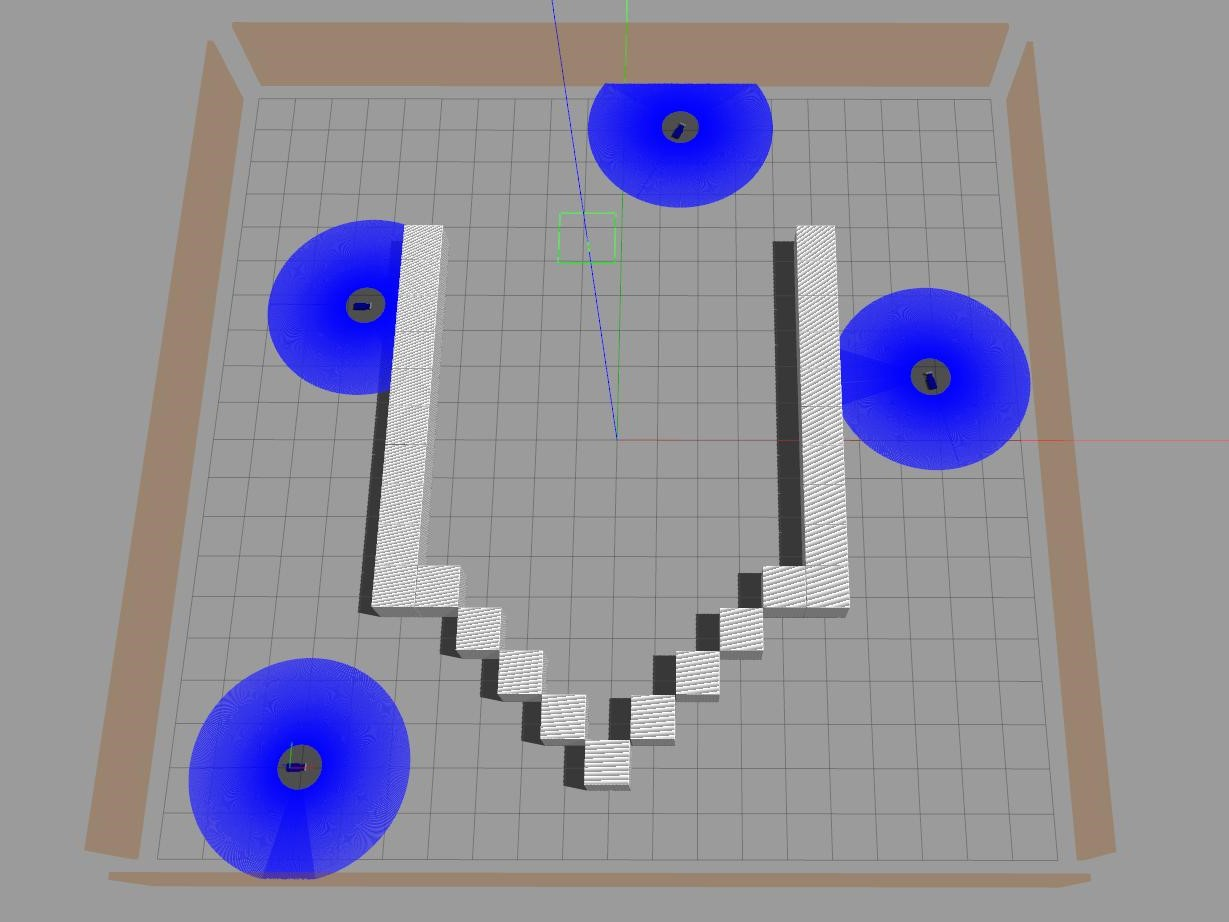
\includegraphics[width=0.24\linewidth]{figs/exp-gazebo.jpg}
    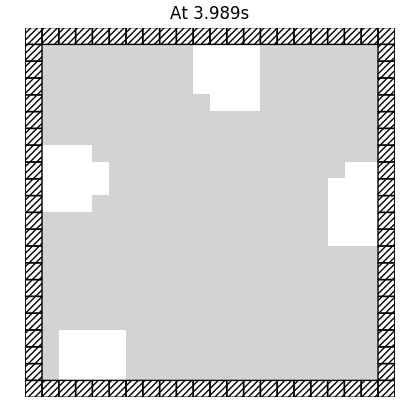
\includegraphics[width=0.24\linewidth]{figs/exp-progress-1.png}
    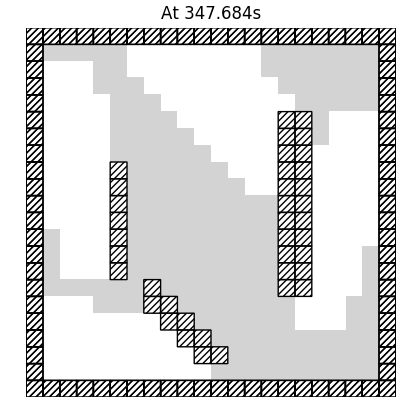
\includegraphics[width=0.24\linewidth]{figs/exp-progress-2.png}
    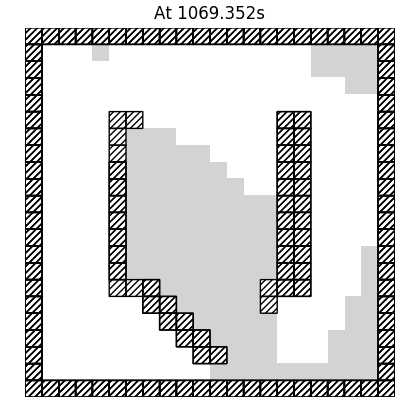
\includegraphics[width=0.24\linewidth]{figs/exp-progress-3.png}
    \caption{Four cars in U-shape world in simulator~(\emph{Left}). Visualization of the global map at three different time stamps~(\emph{Right})}\label{fig:U-map-progress}
\end{figure}

\begin{figure}[t]
    \two{0.4}{0.6}
    {
        \lstinputlisting[language=NumKoord, lastline=25]{code/mapapp.tex}
    }
    {
        \lstinputlisting[language=NumKoord, firstline=26, firstnumber=26]{code/mapapp.tex}
    }
    \caption{$\lgname$ code for Distributed Mapping Application \DMap}
    \label{fig:mapapp}
\end{figure}

\newcommand{\MotionWithScan}{\emph{MotionWithScan}\xspace}
\newcommand{\chk}{\ensuremath{\mathit{chk}}\xspace}

\DMap algorithm works in the following manner.
Each robot constructs a \emph{local grid map} over $D$ using sensors,
and updates it using information from other robots shared via a \emph{global grid map}.
In \reffig{mapapp}, the \MotionWithScan module provides a $\mathit{pscan}$ sensor used to read the LIDAR scan of the actual robot.
The other sensors and actuators {\it position, reached, planner, path} have the same functionality as that in the \Motion module.
The shared allwrite variable $\gmap$ is used to construct a shared map of obstacles within the domain $D$,
and has type $\mathit{GridMap}$, which is a 2-D array representing a grid over $D$.
The local variable $\lmap$ represents each robot's \emph{local} knowledge of the domain $D$, and has the same type as $D$.
There are three \emph{events}: \emph{NewPoint, LUpdate}, and \emph{GUpdate}.
A robot executing the \emph{NewPoint} event, finds an unoccupied point to move to using a user defined function $\mathit{pickFrontierPos}$
and plans a path to it using $\mathit{MotionWithScan.planner}$.
It then updates its $\lmap$ from the shared variable $\gmap$.
The $\mathit{LUpdate}$ event updates the $\lmap$ with scanned sensor data while the robot is in motion,
and the $\mathit{GUpdate}$ event updates the shared $\gmap$ with the updated $\lmap$ information corresponding to the scanned data.

A correctness requirement for \DMap is to ensure that, at any time,
the global grid map $\gmap$ and all local maps $\lmap_i$ should be consistent with the ground truth.
To formally define this requirement as an invariant, we first introduce some auxiliary functions.
Each grid map essentially maps a set $\qdom \subseteq D$ to 0 or 1 based on its occupancy,
where $\qdom$ is a quantized representation of $D$.
For example, we can use $D=\reals^2$ and $Q=\integers^2$ in a 2D world.
Suppose there is a \emph{ground truth} function $\world_Q : Q \mapsto \{0, 1\}$ that gives the actual occupancy of obstacles in this quantized area.
That is, $\forall q \in Q$,
\[
    \world_Q(q) =
    \begin{cases}
        1, & \text{if $q$ is occupied}\\
        0, & \text{otherwise}
    \end{cases}
\]
We can define a function $\chk: GridMap \mapsto \mathbb{B}$ such that
$\chk(g) := \forall q \in Q, (g(q) = 1) \Rightarrow (\world_Q(q) = 1)$ to make sure the detected occupied grids are consistent.
We then can formally define the invariant as:
\begin{invariant}
    \label{inv:mapping}
    $I := \bigwedge\limits_{i \in \UINS} \chk(\lmap_i) \land \chk(\gmap)$
\end{invariant}

For the \emph{NewPoint} event, the post event configuration for robot $i$ is
\[
E_{NP}:= \neg\mathit{on\_path} \land \lmap_i' = \gmap \land \gmap' = \gmap \land \dots
\]
Here we skip the updates of all other variables because they do not appear in \inv{inv:mapping}.
Surprisingly, the \portasum $A$ for this case simply requires the program variables unchanged.
\begin{assumption}
\[
    A := \gmap'' = \gmap' \land \bigwedge\limits_{i \in \UINS} \lmap_i'' = \lmap_i'
\]
\end{assumption}
We skip the proof obligation \PO{po:port-asm} for $A$ because it is trivial.
$I$ is exactly as \inv{inv:mapping}, and similar $I''$ is the primed version.
\PO{po:ind} for the \emph{NewPoint} event is
\begin{proofob}
\(
\bigwedge\limits_{i\in \UINS} I \land E_{NP} \land A \Rightarrow I''
\)
\end{proofob}

For the event \emph{GUpdate},
a \funcasum for the $\mathit{merge}$ function is required.
We simply provide a summary $\mathit{MERGE}$ stating that
the $\mathit{merge}$ function returns a map satisfying $\chk$ when given two maps satisfying $\chk$.

\begin{summary}
\[
\mathit{MERGE}(m_1, m_2, m') := \chk(m_1) \land \chk(m_2) \Rightarrow \chk(m')
\]
\end{summary}
\noindent
The specific proof obligation then is to prove the following:
\begin{proofob}
    \label{merge}
    \[
    \forall m1, m2, MERGE(m1, m2, merge(m1, m2))
    \]
\end{proofob}
\noindent
We then get the post event configuration for robot $i$ as
\[
E_G :=
    \begin{array}{l}
        \mathit{M.reached} \\
        \land\ \mathit{MERGE}(\gmap, \lmap_i, \gmap') \\
        \land \neg on\_path'\land\ \lmap_i' = \lmap_i \land \dots \\
    \end{array}
\]
$I, I''$, and $A$ are the same as those for the \emph{NewPoint} event.
The overall constraint for this event along with its precondition is therefore:
\begin{proofob}
\(
\bigwedge_{i\in \UINS} I \land E_G \land A \Rightarrow I''
\)
\end{proofob}

We omit the discussion for \emph{LUpdate} in the interest of space,
as it follows along the lines of the previous constraints.
It requires an additional proof obligation on the $\mathit{scanToMap}$ function and the consistency of the sensor data $\mathit{M.pscan}$ with the ground truth,
along with unrolling the \emph{for-loop} to the number of sensor observations.
The overall induction proof obligation is a conjunction of the three.

Table~\ref{tab:map} summarizes the verification of these constraints on systems of different $\NMAX$ .
\begin{table}

    \scriptsize
 \centering
   \begin{tabular}{ l|  c c c c  }
 \hline
 \tb{Benchmark}       & \tb{robots}(N) & $T_K$ (s) & $T_V$ (s)   & \qquad\tb{Safe\ \ \ \ } \\ \hline
 \dmap       & 3     &  &   & \Checkmark  \\
 \dmap      & 4      &  &  & \Checkmark   \\
 \dmap       & 5      &  &  & \Checkmark   \\
\dmap        & 10     &   &   & \Checkmark  \\
\end{tabular}
    \caption{ \small Summary of semantics based verification for \dmap.  $T_K$ is the symbolic post computation time in \K, $T_V$ is the time taken for generation of constraints and verification in Z3 and \emph{robots}(N) is the number of robots in the system.}\label{tab:map}
\end{table}

